
\graphicspath{{figures/powerlog/}}
\chapter{Powers and Logarithms}\label{app power log}





\section{Powers}\label{sec powers}
In the following, $x$ and $y$ are arbitrary real numbers,
$q$ is an arbitrary constant that is strictly bigger
than zero and $e$ is 2.7182818284, to ten decimal places.
\begin{itemize}
 \item 
     $e^0=1$,\quad $q^0=1$

\item 
         $e^{x+y}=e^xe^y$,\quad
         $e^{x-y}=\frac{e^x}{e^y}$,\quad
         $q^{x+y}=q^xq^y$,\quad
         $q^{x-y}=\frac{q^x}{q^y}$


\item 
   $e^{-x}=\frac{1}{e^x}$,\quad
   $q^{-x}=\frac{1}{q^x}$

\item 
    $\big(e^x\big)^y=e^{xy}$,\quad
    $\big(q^x\big)^y=q^{xy}$
\item 
    $\diff{\hfill}{x}e^x=e^x$,\quad
    $\diff{\hfill}{x}e^{g(x)}=g'(x)e^{g(x)}$,\quad
    $\diff{\hfill}{x}q^x=(\ln q)\ q^x$
\item
    $\int e^x\ \dee{x}=e^x+C$,\quad
    $\int e^{ax}\ \dee{x}=\frac{1}{a}e^{ax}+C$ if $a\ne 0$
\item
     $e^x =\sum\limits_{n=0}^\infty\frac{x^n}{n!}$
\item    
    $\lim\limits_{x\rightarrow\infty}e^x=\infty$, \quad
    $\lim\limits_{x\rightarrow-\infty}e^x=0$ 

    $\lim\limits_{x\rightarrow\infty}q^x=\infty$, \quad
    $\lim\limits_{x\rightarrow-\infty}q^x=0$ if $q>1$

    $\lim\limits_{x\rightarrow\infty}q^x=0$, \quad
    $\lim\limits_{x\rightarrow-\infty}q^x=\infty$ if $0<q<1$
\item  The graph of $2^x$ is given below. The graph of  $q^x$,
for any $q>1$, is similar.

\begin{center}
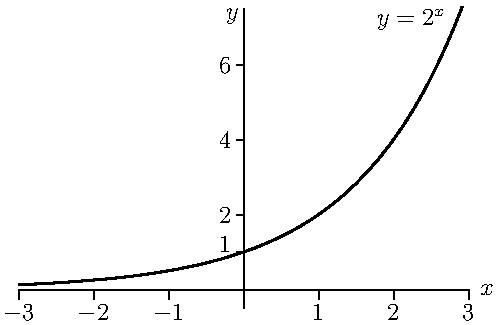
\includegraphics{expGraph2.pdf}
\end{center}


\end{itemize}


\section{Logarithms}\label{sec logs}

In the following, $x$ and $y$ are arbitrary real numbers that 
are strictly bigger than 0 (except where otherwise specified), 
$p$ and $q$ are arbitrary constants that are strictly bigger 
than one, and $e$ is 2.7182818284, to ten decimal places.
The notation $\ln x$ means $\log_e x$. Some people use $\log x$
to mean $\log_{10} x$, others use it to mean $\log_e x$ and still
others use it to mean $\log_2 x$.

\begin{itemize}
\item   
       $e^{\ln x}=x$,\quad  
       $q^{\log_q x}=x$
\item 
       $\ln \big(e^x\big)=x$,\quad
       $\log_q \big(q^x\big)=x$\quad for all $-\infty<x<\infty$ 
\item   
        $\log_q x=\frac{\ln x}{\ln q}$,\quad
        $\ln x=\frac{\log_p x}{\log_p e}$,\quad
        $\log_q x=\frac{\log_p x}{\log_p q}$
\item   
          $\ln 1=0$,\quad 
          $\ln e=1$


          $\log_q 1=0$,\quad 
          $\log_q q=1$

\item 
      $\ln(xy)=\ln x+\ln y$,\quad
      $\log_q(xy)=\log_q x+\log_q y$

\item 
     $\ln\big(\frac{x}{y}\big)=\ln x-\ln y$,\quad 
     $\log_q\big(\frac{x}{y}\big)=\log_q x-\log_q y$
 
\item 
     $\ln\big(\frac{1}{y}\big)=-\ln y$,\quad 
     $\log_q\big(\frac{1}{y}\big)=-\log_q y$

\item 
     $\ln(x^y)=y\ln x$,\quad
     $\log_q(x^y)=y\log_q x$

\item
    $\diff{\hfill}{x}\ln x = \frac{1}{x}$,\quad
    $\diff{\hfill}{x}\log_q x = \frac{1}{x\ln q}$

\item
    $\int \ln x\ \dee{x}= x\ln x-x +C$,\quad
    $\int \log_q x\ \dee{x}= x\log_q x-\frac{x}{\ln q} +C$,\quad

\item
    $\lim\limits_{x\rightarrow\infty}\ln x=\infty$,\quad 
           $\lim\limits_{x\rightarrow0}\ln x=-\infty$

    $\lim\limits_{x\rightarrow\infty}\log_q x=\infty$,\quad
           $\lim\limits_{x\rightarrow0}\log_q x=-\infty$ 

\item The graph of $\log_{10} x$ is given below. The graph of  $\log_q x$,
for any $q>1$, is similar.

\begin{center}
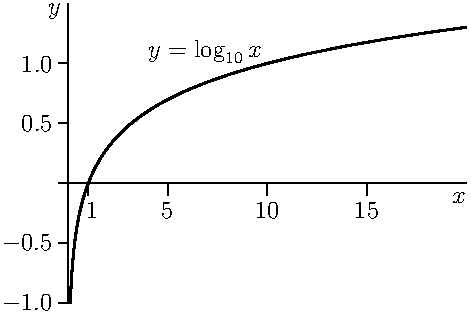
\includegraphics{logGraph10.pdf}
\end{center}

\end{itemize}






